\section{}

% Plot all the collected data (displacement vs voltage) for the potentiometer and
% find the correlating function with a function of the form x=aV+b. Report the equation used 
% in the fit of your data. Determine the sensitivity and span.

\subsection{}
% slope	12.672	-1.499	intercept
% r^2	1.000

The plot of displacement over voltage can be found in Fig. \ref{fig:Q1a}. The slope, intercept, and $R^2$ value of the linear regression 
were determined using \texttt{=LINEST()} in Excel. The results can be found in Table \ref{tab:Q1a}.

\begin{table}[h]
    \centering
    \caption{Linear regression of displacement over voltage}
    \label{tab:Q1a}
    \begin{tabular}{ccc}
        \hline
        Slope & Intercept & $R^2$ \\
        (mm/V) & (mm) & \\
        \midrule
        12.67 & -1.50 & 1.00 \\
        \hline
    \end{tabular}
\end{table}

\begin{figure}[h]
    \centering
    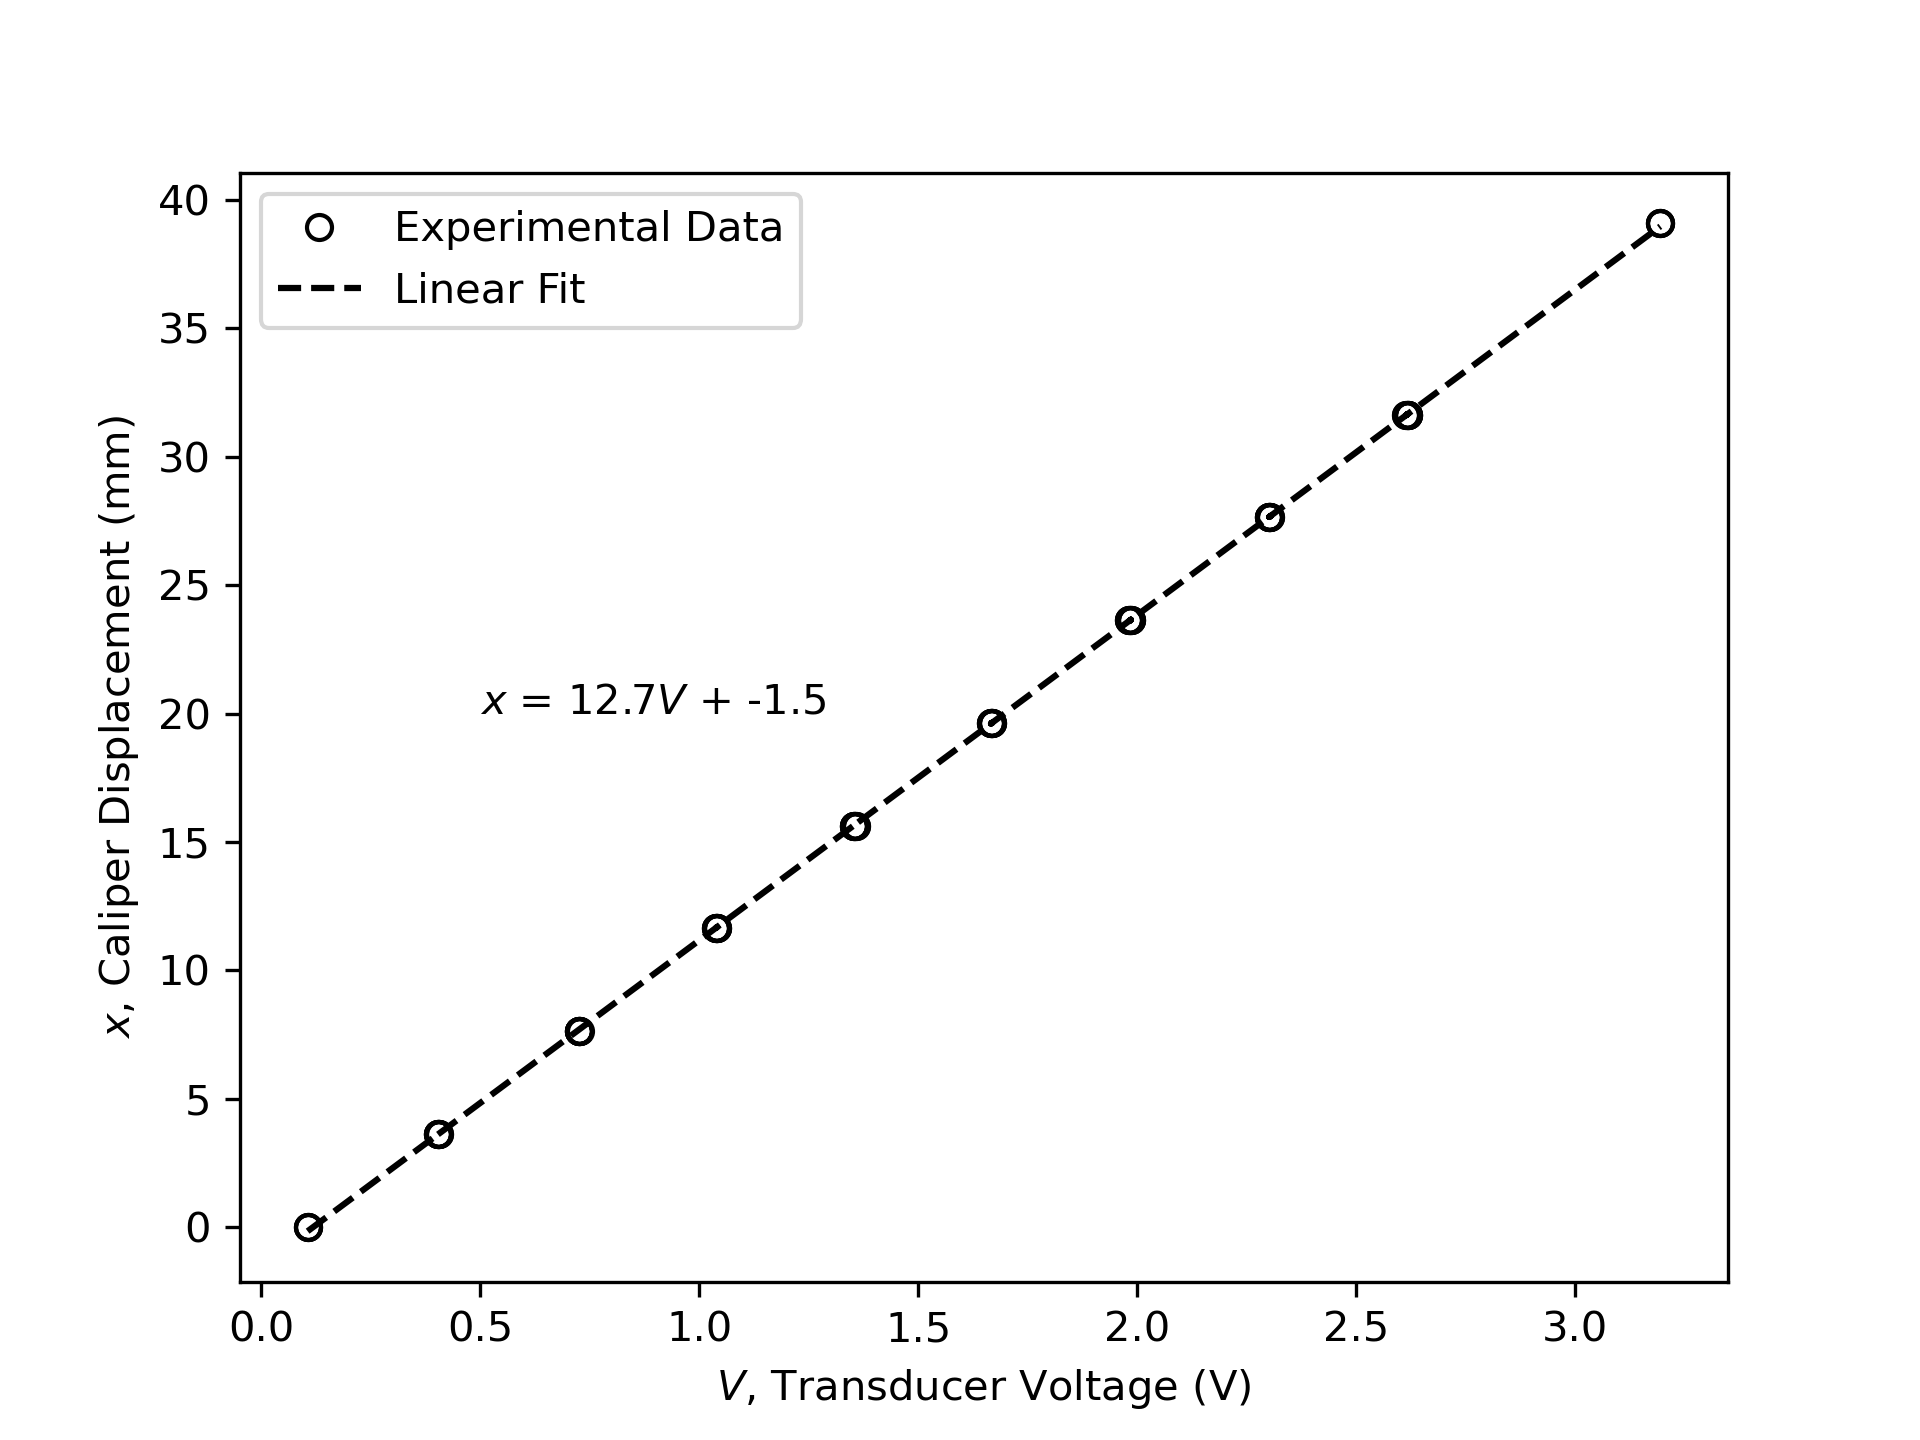
\includegraphics[width=0.8\linewidth]{matplotlib/Q1a.png}
    \caption{Displacement over voltage for the potentiometer}
    \label{fig:Q1a}
\end{figure}

Note that 2 decimal places were chosen as linear regression involved sum of squares, and the limiting
decimal place was 2, which comes from the caliper measurements.

The function is:
\begin{equation}
    \boxed{x = 12.67V - 1.50  \;\;[\unit[]{mm}]} \label{eq:Q1a}
\end{equation}

The sensitivity is the inverse of the slope, 
\[\boxed{\text{Sensitivity} = \frac{1}{12.67} = \qty{0.07891}{\milli\meter\per\volt}}\]

The span is the difference between the maximum and minimum displacement. The span is therefore,
\[\boxed{\text{Span} = \qty{39.10}{\milli\meter}}\]


\subsection{}
% b) Make a deviation table, deviation curve, linearity table (independent linearity 
% only), and hysteresis table. Use units of mm.

First, all the voltages were converted to displacements using the linear regression function, Eq. (\ref{eq:Q1a}) discussed in the previous section. The
displacement table can be found in Appendix \ref{sec:appendix-potentiometer-displacement-table} in Table \ref{tab:appendix-potentiometer-displacement-table}.

The deviation table can be found in Table \ref{tab:Q1b-deviation-table}. The deviation curve can be found in Fig. \ref{fig:Q1b-deviation-curve}.

\begin{table}[h]
    \centering
    \caption{Deviation table of potentiometer after conversion to displacement.}
    \label{tab:Q1b-deviation-table}
    \begin{tabular}{ccccccc}
        \hline
        Caliper Reading & Up 1 & Down 1 & Up 2 & Down 2 & Up 3 & Down 3 \\
        (mm) & (mm) & (mm) & (mm) & (mm) & (mm) & (mm) \\
        \midrule
        0.00 & & -0.16 & & -0.16 & & -0.16 \\
        3.64 & -0.03 & -0.03 & -0.03 & 0.01 & -0.03 & 0.01 \\
        7.64 & 0.05 & 0.05 & 0.05 & 0.05 & 0.05 & 0.09 \\
        11.64 & 0.05 & 0.05 & 0.05 & 0.02 & 0.02 & 0.02 \\
        15.64 & 0.06 & 0.02 & 0.02 & 0.02 & 0.02 & 0.06 \\
        19.64 & 0.01 & 0.01 & -0.03 & -0.03 & 0.01 & -0.03 \\
        23.64 & 0.02 & -0.02 & 0.02 & -0.02 & 0.02 & -0.02 \\
        27.64 & 0.06 & 0.02 & 0.02 & 0.02 & 0.06 & 0.02 \\
        31.64 & 0.03 & -0.01 & 0.03 & -0.01 & 0.03 & 0.03 \\
        39.10 & -0.12 & & -0.12 & & -0.12 \\
        \hline
    \end{tabular}
\end{table}

\begin{figure}[h]
    \centering
    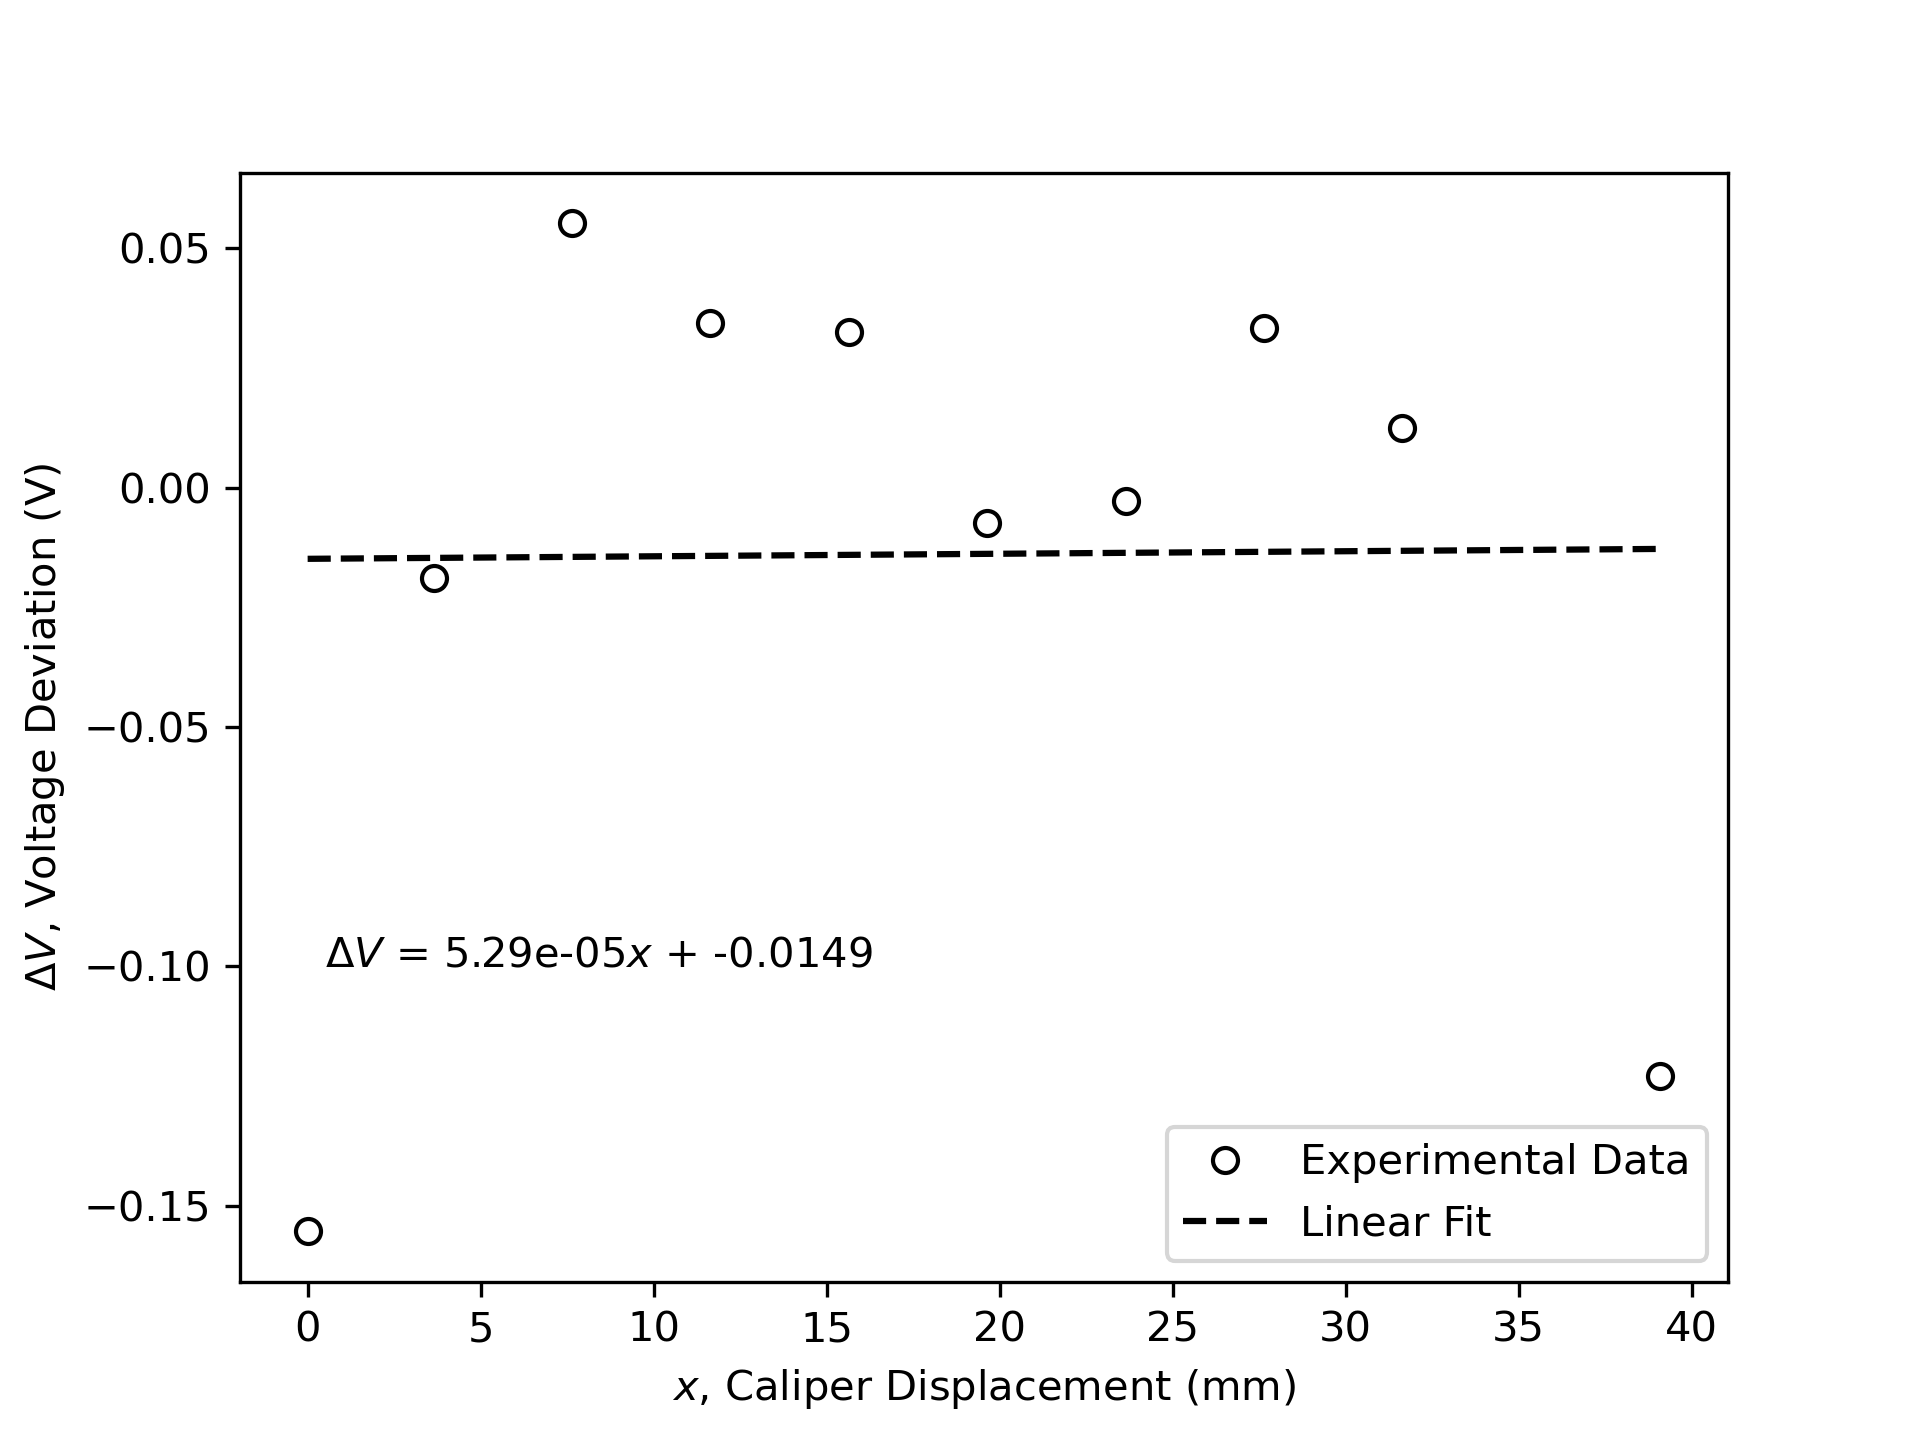
\includegraphics[width=0.8\linewidth]{matplotlib/Q1b.png}
    \caption{Displacement deviation curve of potentiometer with respect to displacement (independent linearity).}
    \label{fig:Q1b-deviation-curve}
\end{figure}

The linear fit for the deviation curve was found by using \texttt{=LINEST()} in Excel. The results can be found in Table \ref{tab:Q1b-deviation-curve-linear-fit}.

\begin{table}[h]
    \centering
    \caption{Linear fit of deviation curve of potentiometer with respect to displacement (independent linearity).}
    \label{tab:Q1b-deviation-curve-linear-fit}
    \begin{tabular}{ccc}
        \hline
        Slope & Intercept & $R^2$ \\
        (V/mm) & (V) & \\
        \midrule
        5.29E-05 & -1.49E-02 & 9.11E-05 \\
        \hline
    \end{tabular}
\end{table}

The fit function for deviation is therefore,
\[\Delta x = 5.29 \times 10^{-5}x - 1.49 \times 10^{-2} \;\;[\unit[]{mm}]\]

Evaluating the fit function at all displacements results in difference deviation Table \ref{tab:Q1b-diff-deviation-table}.
\begin{table}[h]
    \centering
    \caption{Difference table of nominal deviation and linear fit of deviation.}
    \label{tab:Q1b-diff-deviation-table}
    \begin{tabular}{cccc}
        \hline
        Caliper Reading & Nominal Deviation & Independent Fit & Difference \\
        (mm) & (mm) & (mm) & (mm) \\
        \midrule
        0.00 & -0.16 & -0.015 & {0.14} \\
        3.64 & -0.03 & -0.015 & 0.00 \\
        7.64 & 0.05 & -0.014 & -0.07 \\
        11.64 & 0.05 & -0.014 & -0.05 \\
        15.64 & 0.06 & -0.014 & -0.05 \\
        19.64 & 0.01 & -0.014 & -0.01 \\
        23.64 & 0.02 & -0.014 & -0.01 \\
        27.64 & 0.06 & -0.013 & -0.05 \\
        31.64 & 0.03 & -0.013 & -0.03 \\
        39.10 & -0.12 & -0.013 & 0.11 \\
        \hline
    \end{tabular}
\end{table}

A hysteresis table can be generated by subtracting the up and down readings. The hysteresis table can be found in Table \ref{tab:Q1b-hysteresis-table}.
\begin{table}[h]
    \centering
    \caption{Hysteresis table of potentiometer.}
    \label{tab:Q1b-hysteresis-table}
    \begin{tabular}{cccc}
        \hline
        Caliper Reading & Up 1 - Down 1 & Up 2 - Down 2 & Up 3 - Down 3 \\
        (mm) & (mm) & (mm) & (mm) \\
        \midrule
        3.64 & 0.00 & -0.04 & -0.04 \\
        7.64 & 0.00 & 0.00 & -0.04 \\
        11.64 & 0.00 & 0.04 & 0.00 \\
        15.64 & 0.04 & 0.00 & -0.04 \\
        19.64 & 0.00 & 0.00 & 0.04 \\
        23.64 & 0.04 & 0.04 & 0.04 \\
        27.64 & 0.04 & 0.00 & 0.04 \\
        31.64 & 0.04 & 0.04 & 0.00 \\
        \hline
    \end{tabular}
\end{table}
\FloatBarrier

\subsection{}

% c) Determine the accuracy, repeatability, linearity (independent), resolution, and 
% hysteresis, in units of mm and % output span. 

A summary table is provided below:
\begin{table}[h]
    \centering
    \caption{Summary of results for potentiometer.}
    \label{tab:Q1c-summary-table}
    \begin{tabular}{ccc}
        \hline
        & Nominal & Relative \\
        & (mm) & (\%) \\
        \midrule
        Accuracy & $\pm$ 0.16 & $\pm$ 0.40 \\
        Repeatability & $\pm$ 0.04 & $\pm$ 0.10 \\
        Linearity & 0.14 & 0.36 \\
        Resolution & 0.038 & 0.097 \\
        Hysteresis & 0.04 & 0.10 \\
        \hline
    \end{tabular}
\end{table}

Accuracy can be found by taking the max value absolute value of the deviation Table \ref{tab:Q1b-deviation-table}. The accuracy is therefore,
\[\boxed{\text{Accuracy} = \max(\text{Table}) = \pm \qty{0.16}{\milli\meter}}\]

Relative accuracy is
\[\boxed{\text{Relative Accuracy} = \frac{\text{Accuracy}}{\text{Span}} = \frac{0.16}{39.10} = \pm 0.40\%}\]    

The repeatability is simply the maximum deviation between repeated measurements of the same caliper reading approached from the same direction.
\begin{empheq}[box=\fbox]{align*}
    \text{Repeatability} &= \max(\text{Table}) \\
    &= \max \left(
    \begin{bmatrix}
        0.00 & 0.00 \\
        0.00 & 0.04 \\
        0.04 & 0.04 \\
        0.04 & 0.04 \\
        0.04 & 0.04 \\
        0.00 & 0.04 \\
        0.04 & 0.00 \\
        0.00 & 0.00 \\
        0.00 & 0.04 \\
    \end{bmatrix}
    \right)
    \\
    &= \pm\qty{0.04}{\milli\meter} 
\end{empheq}

The relative repeatability is
\[\boxed{\text{Relative Repeatability} = \frac{\text{Repeatability}}{\text{Span}} = \frac{0.04}{39.10} = \pm 0.1\%}\]

The linearity is the maximum difference between the nominal deviation and the linear fit of the deviation. The linearity is therefore,
\begin{empheq}[box=\fbox]{align*}
    \text{Linearity} &= \max(\text{Table}) \\
    &= \max \left(
    \begin{bmatrix}
        0.14 \\
        0.00 \\
        -0.07 \\
        -0.05 \\
        -0.05 \\
        -0.01 \\
        -0.01 \\
        -0.05 \\
        -0.03 \\
        0.11 \\
    \end{bmatrix}
    \right)
    \\
    &= \qty{0.14}{\milli\meter}
\end{empheq}

The relative linearity is
\[\boxed{\text{Relative Linearity} = \frac{\text{Linearity}}{\text{Span}} = \frac{0.14}{39.10} = 0.36\%}\]

A resistor is a transducer that converts electrical energy to heat energy. The resolution of a transducer is
\[{\text{Resolution} = \frac{V_\text{Span}}{2^n G\eta}}\]
where $G$ is the gain, and $\eta$ is the sensitivity. The resolution of this system is therefore,
\[\boxed{\text{Resolution} = \frac{3.3}{2^{10} \times 1 \times 0.07891} = \qty{0.038}{\volt}}\]

The relative resolution is
\[\boxed{\text{Relative Resolution} = \frac{\text{Resolution}}{\text{Span}} = \frac{0.038}{39.10} = 0.097\%}\]

The hysteresis is the maximum difference between the up and down readings. The hysteresis can be found by applying \texttt{{=MAX(ABS(Table))}} in Excel on 
Table \ref{tab:Q1b-hysteresis-table}. The hysteresis is therefore,
\[\boxed{\text{Hysteresis} = \qty{0.04}{\milli\meter}}\]

The relative hysteresis is
\[\boxed{\text{Relative Hysteresis} = \frac{\text{Hysteresis}}{\text{Span}} = \frac{0.04}{39.10} = 0.1\%}\]

\subsection{}
% Make a plot of the displacement of the potentiometer (mm) as a function of time 
% (s) when it was connected to the servo motor. Define the first measurement point as t=0 s.
% Make a plot of velocity of the potentiometer (mm/s) as a function of time (s). Explain how 
% you calculated velocity.

The plot of displacement over time and velocity over time can be found in Fig. \ref{fig:Q1d-displacement} and Fig. \ref{fig:Q1d-velocity} respectively.

\begin{figure}[h]
    \centering
    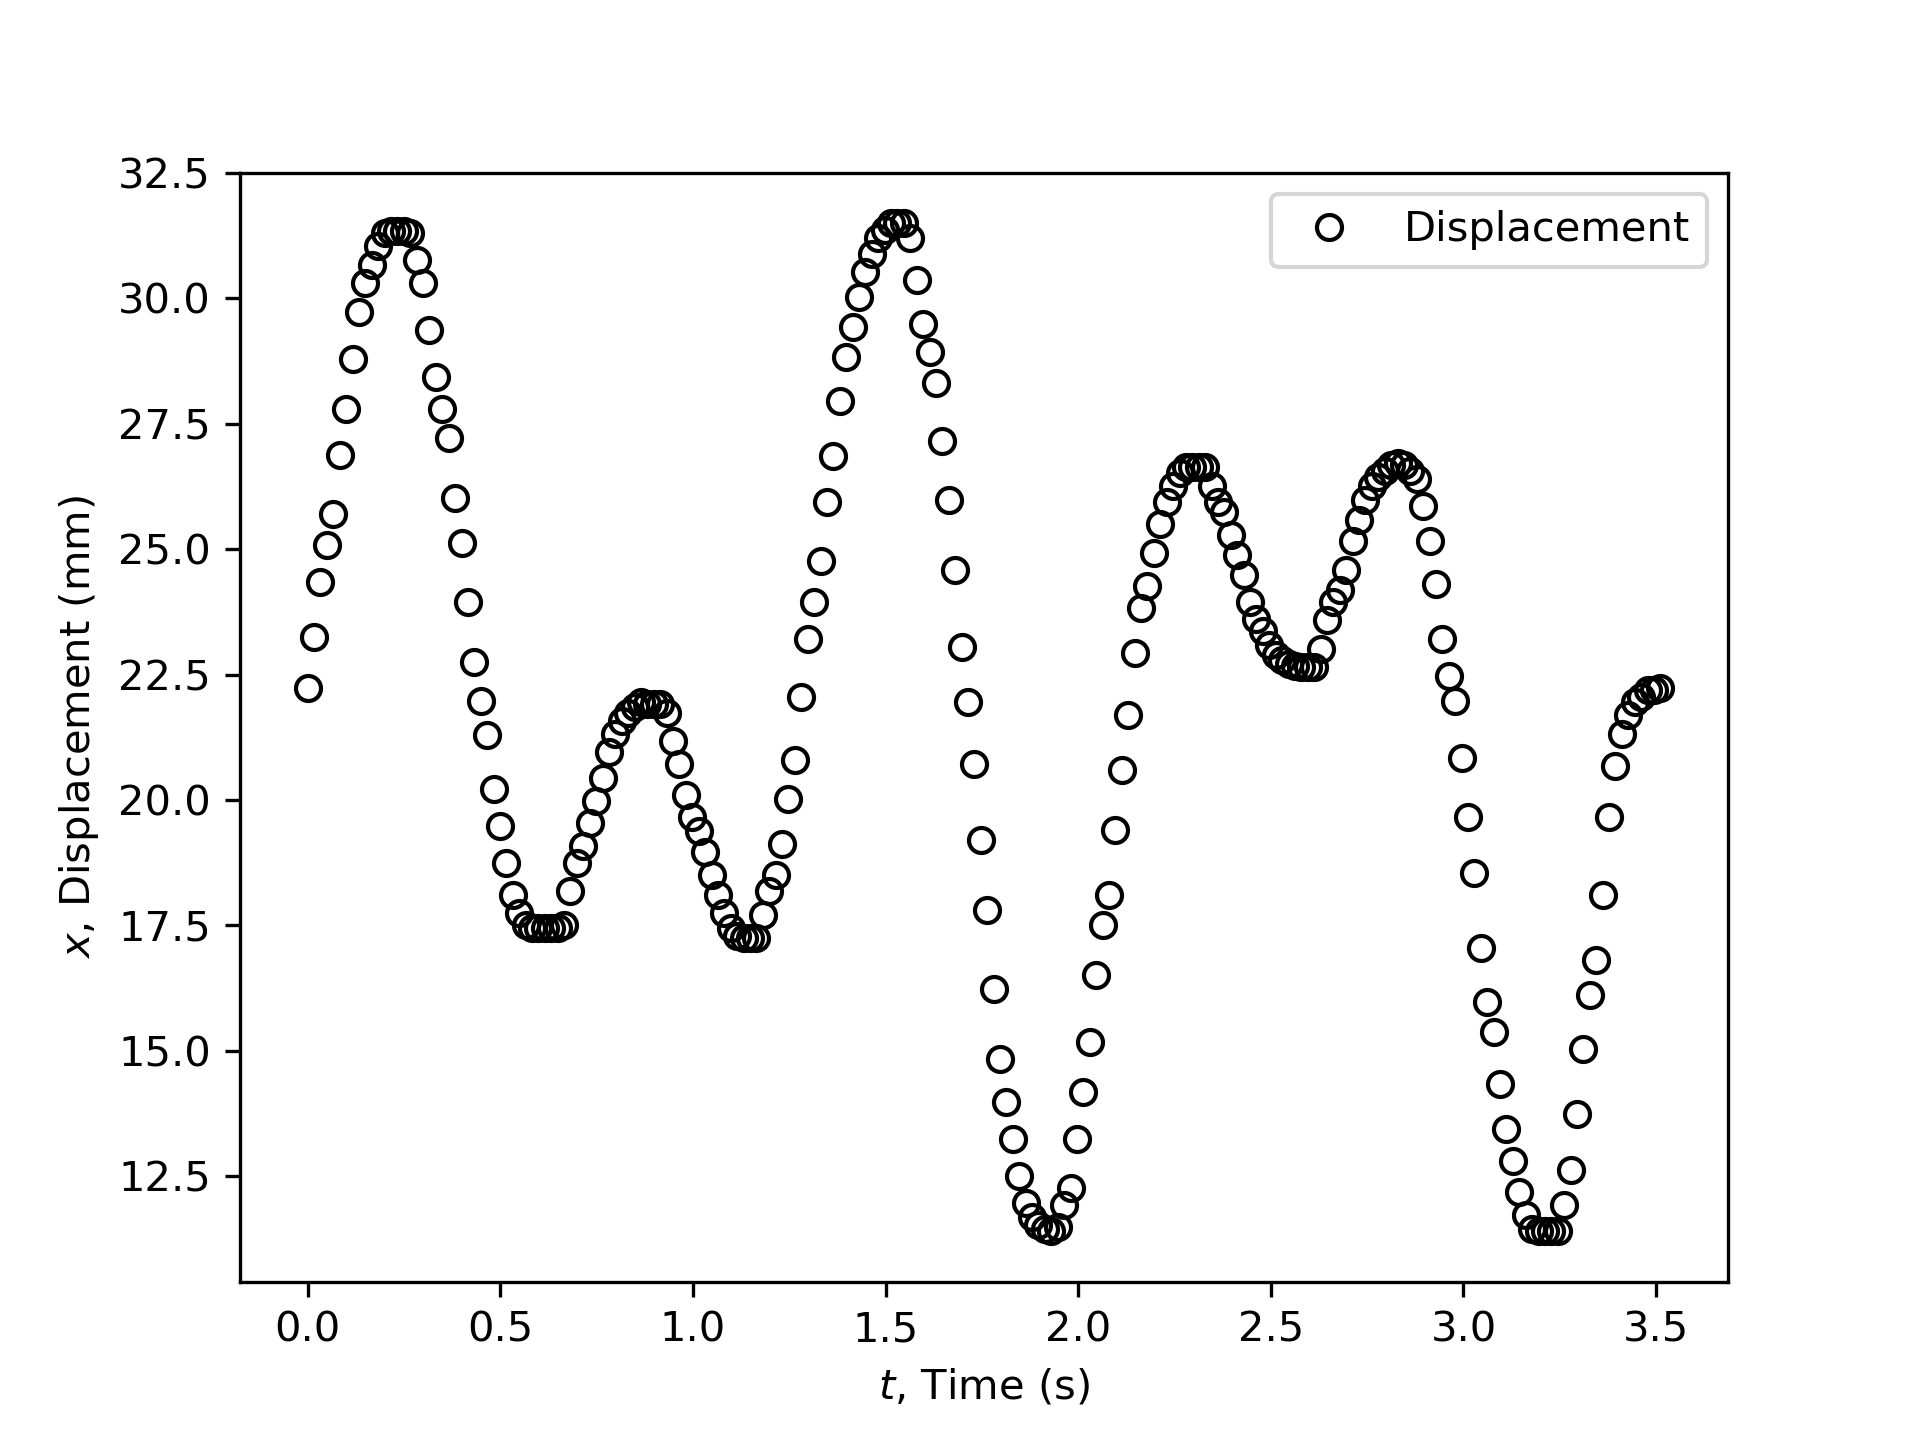
\includegraphics[width=0.8\linewidth]{matplotlib/Q1cDisplacement.png}
    \caption{Displacement over time of potentiometer.}
    \label{fig:Q1d-displacement}
\end{figure}

\begin{figure}[h]
    \centering
    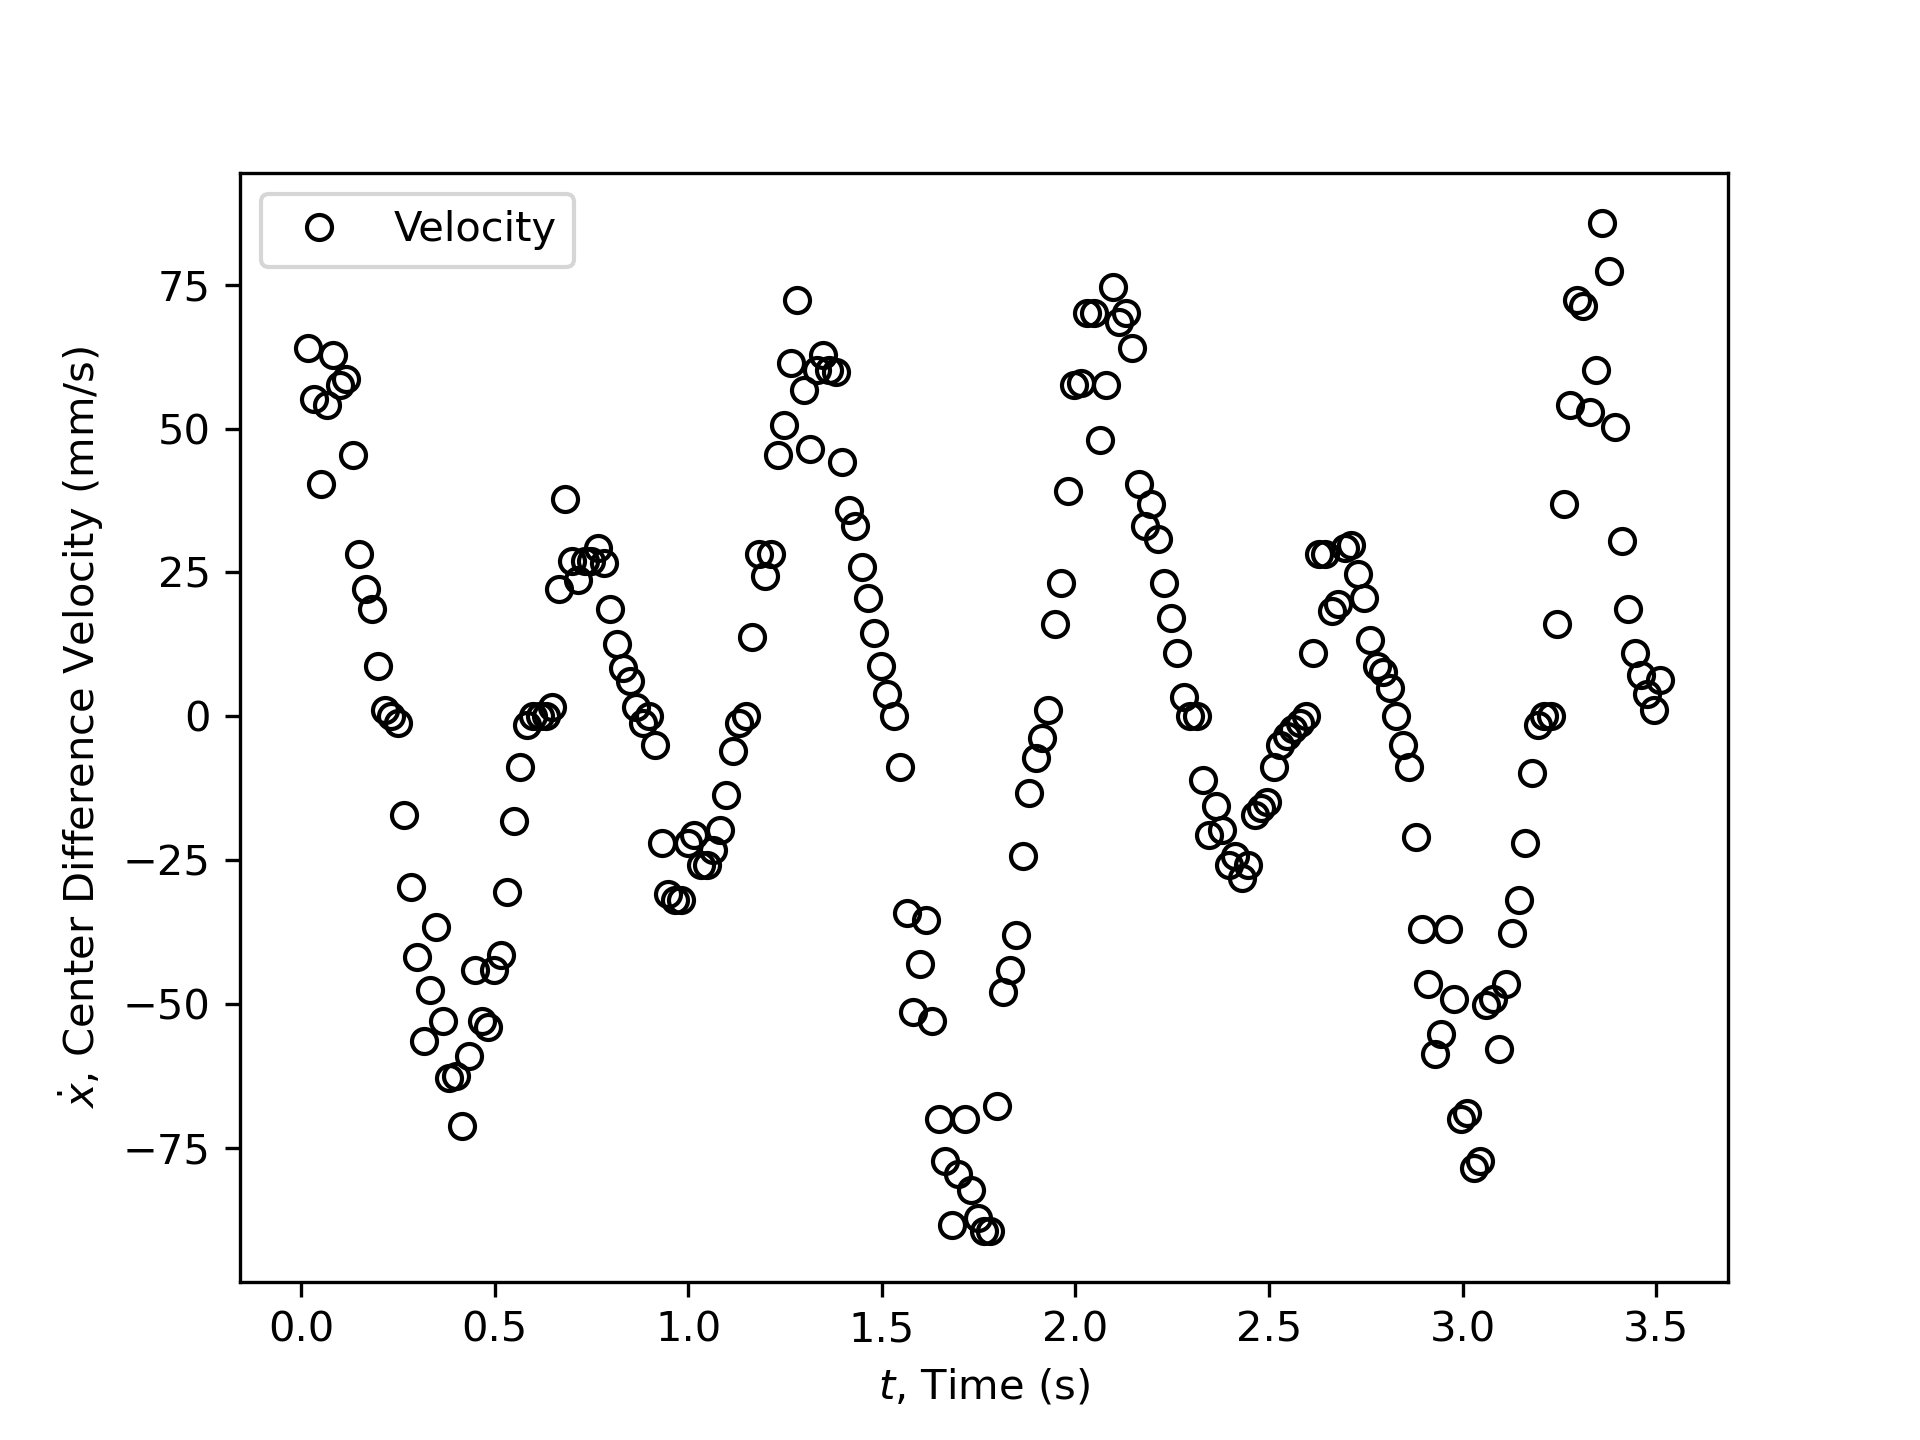
\includegraphics[width=0.8\linewidth]{matplotlib/Q1cVelocity.png}
    \caption{Velocity over time of potentiometer.}
    \label{fig:Q1d-velocity}
\end{figure}

The velocity was calculated by taking the central difference of the displacement. This was chosen because
the central difference method has an error of $O(h^2)$, whereas the forwards and backwards difference methods have an error of $O(h)$. A downside
is that the first and last points cannot be calculated. However, due to the large number of points, this was negligible.


    